\documentclass[12pt,oneside,a4paper,notitlepage]{report}

\usepackage[backend=biber,sorting=none,maxbibnames=99]{biblatex}
\usepackage{setspace}
\usepackage{graphicx}
\usepackage{syntax}
%\usepackage{wasysym}
\usepackage{textcomp}
\usepackage{newfloat}
\usepackage{enumitem}
\usepackage{listings}

\title{
	Implementing an Object Model for TDL\textsuperscript{TP} Expressions
}
\author{Tanel Prikk}

\DeclareFloatingEnvironment[
fileext   = logr,
listname  = {List of Grammars},
name      = Grammar,
placement = htp
]{GrammarWrapper}
\setlength{\grammarindent}{5em}
\setlength{\grammarparsep}{5pt plus 1pt minus 1pt}

\newcommand{\texttilde}{\raisebox{0.5ex}{\texttildelow}}

\addbibresource{Sources.bib}
\pagenumbering{gobble}
\singlespacing


\begin{document}
	\maketitle

	\section*{Background}
	\par Our ANTLR-generated parser is capable of building parse trees for TDL\textsuperscript{TP} expressions. The object structure of said trees is, however, dependent on the ANTLR library. Higher-level components that will work with TDL parse trees should be decoupled from this implementation detail. To achieve this, we define an independent object model which provides facilities for storage and traversal of TDL parse trees. In the future, we will also write adapter logic for converting ANTLR TDL parse trees to objects from our independent object model.

	\newpage

	\section*{Requirements Analysis}
	\par Considering that we need to work with a parse tree (concrete syntax tree, henceforth expression tree), a suitable data structure for storing this is a rooted ordered tree. A classical implementation of such a tree is pointer-based. We provide a class diagram below:

	\begin{figure}[h]
		\begin{center}
		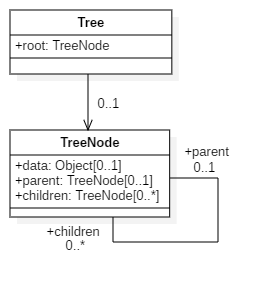
\includegraphics{Models/BasicTree}
		\end{center}
		\caption{Tree class diagram.}
		\label{fig:basic-tree}
	\end{figure}

	\par A simple approach would directly utilize the tree data structure from figure~\ref{fig:basic-tree} and provide implementations for each possible expression node that may occur in an abstract expression tree. 
	However, this is too inconvenient for clients to work with. A better approach is to take the basic \texttt{Tree} data structure as a basis for a specialized expression tree. We can encode structural rules in the APIs of the objects in an expression tree.

	\newpage

	\par To begin specifying our expression tree object model, we should take into consideration the grammar for the language, reproduced below:

	\begin{GrammarWrapper}
		\begin{grammar}
			% https://tex.stackexchange.com/questions/24886/which-package-can-be-used-to-write-bnf-grammars
			% http://texdoc.net/texmf-dist/doc/latex/mdwtools/syntax.pdf
			<Expression>	::=	'(' <Expression> ')'
			\alt 				'A' '(' <TrapsetExpression> ')'
			\alt 				'E' '(' <TrapsetExpression> ')'
			\alt 				<UnaryOp> <Expression>
			\alt 				<Expression> <BinaryOp> <Expression>
			\alt 				<Expression> '\texttilde' '\textgreater' <Expression> 
			\alt 				<Expression> '\texttilde' '\textgreater' '[' <RelOp> <NUM> ']' <Expression> 
			\alt 				'\#' <Expression> '[' <RelOp> <NUM> ']'
			
			<TrapsetExpression>	::=	'(' <TrapsetExpression> ')'
			\alt						'!' <ID>
			\alt 						<ID> '\textbackslash' <ID>
			\alt						<ID> ';' <ID>
			
			<UnaryOp>	::= '\texttilde'
			
			<BinaryOp>	::= '\&' | '|' | '-' '\textgreater' | '\textless' '-' '\textgreater'
			
			<RelOp> 	::= '\textless' | '=' | '\textgreater' | '\textless' '=' | '\textgreater' '='
			
			<ID> 		::= 'TR' <NUM>
			
			<NUM> 		::= ('0' ... '9')+
		\end{grammar}
		\caption{TDL\textsuperscript{TP} grammar}\label{bnf:modified}
	\end{GrammarWrapper}

	\newpage

	\par We can note the following simplifying factors based on grammar~\ref{bnf:modified}:
	\begin{enumerate}[label=\textbf{\arabic*.},ref=\textit{\arabic*}]
		\item \label{simp-1} instead of treating operators as terminals, we can use them to create operator node types in our data model;
		\item \label{simp-2} the negation operation is applicable for all abstract logical operations - we can treat negation as an attribute for logical operation nodes (which provides a justification for having a grouping of such node types);
		\item \label{simp-3} bound nodes (which, when treated as a whole, are a kind of terminal in TDL expression trees) are only applicable for certain logical operations; we can assume that it will not be necessary to visit such nodes separately - we can move them into the structure of concrete logical operator node types;
		\item \label{simp-4} items \ref{simp-1} and \ref{simp-3} allow us to have the trapset symbol node type as the only leaf node type;
		\item \label{simp-5} items \ref{simp-1} and \ref{simp-3} allow us to have operator node types as the only internal node types;
		\item \label{simp-6} each operator node has a restricted domain of possible operators - this can be used when defining operator node types to encode expectations on operand instances;
		\item \label{simp-7} item \ref{simp-5} allows us to have the trapset operator node type and the logical operator node type as the only variants of an internal node type;
		\item \label{simp-8} all internal operator node types have a minimum arity of 1 and a maximum arity of 2 - this allows us to specify arity contracts which help guide and prevent clients from ignoring arity restrictions;
		\item \label{simp-9} the root node object is always an operator node.
	\end{enumerate}

	\newpage

	\par Based on simplifications \ref{simp-1}, \ref{simp-5}, \ref{simp-6}, and \ref{simp-9} we can construct the following generic expression tree object model:
	
	\begin{figure}[h]
		\begin{center}
			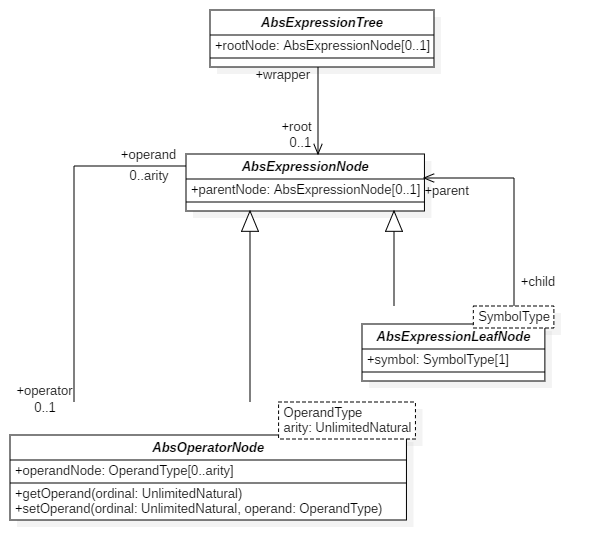
\includegraphics[width=\textwidth]
			{Models/BasicAbstractExpressionTree}
		\end{center}
		\caption{Basic expression tree.}
		\label{fig:basic-expr-tree}
	\end{figure}

	\newpage

	\par Simplifications \ref{simp-2}, \ref{simp-4}, and \ref{simp-7} allow us to encode logical operators and trapset symbol nodes in the model:

	\begin{figure}[h]
		\begin{center}
			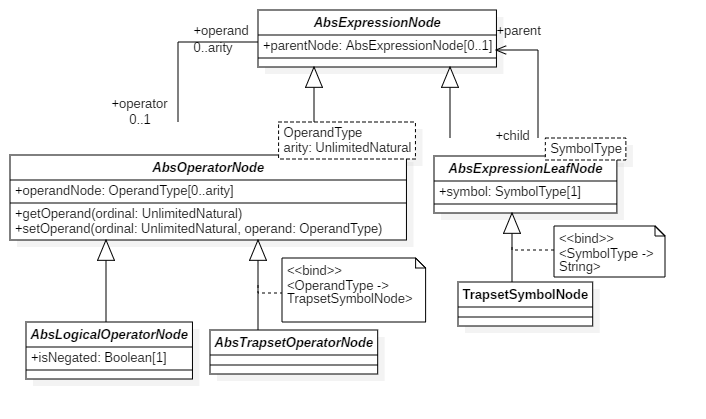
\includegraphics[width=\textwidth]{Models/BasicConcreteExpressionTree}
		\end{center}
		\caption{Model extended with logical and trapset operators.}
		\label{fig:basic-concrete-expr-tree}
	\end{figure}

	\newpage

	\par Now we can utilize \ref{simp-9} and provide a concrete sub-type for \texttt{AbsExpressionTree}:

	\begin{figure}[h]
		\begin{center}
			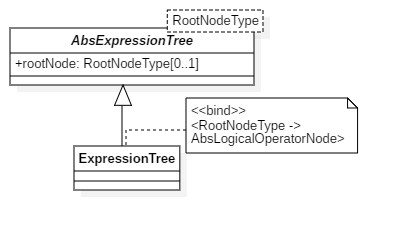
\includegraphics{Models/ExpressionTreeModelFragment}
		\end{center}
		\caption{Expression tree root.}
		\label{fig:expression-tree-model-fragment}
	\end{figure}

	\newpage

	\par Using simplification \ref{simp-6}, we can implement concrete trapset operator types.

	\begin{figure}[h]
		\begin{center}
			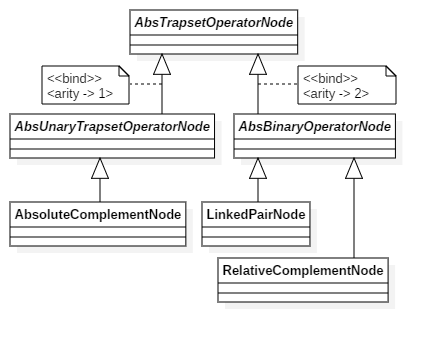
\includegraphics{Models/TrapsetOperatorType}
		\end{center}
		\caption{Trapset operator types.}
		\label{fig:trapset-operator-types}
	\end{figure}

	\newpage

	\par To implement concrete logical operator types, we first define an interface for bounded operators based on simplification \ref{simp-3}:

	\begin{figure}[h]
		\begin{center}
			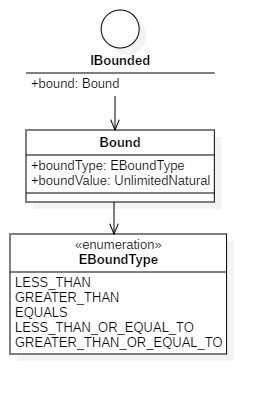
\includegraphics{Models/BoundModifier}
		\end{center}
		\caption{Bound interface.}
		\label{fig:bound-interface}
	\end{figure}

	\newpage

	\par Unary logical operator types are provided below:
	
	\begin{figure}[h]
		\begin{center}
			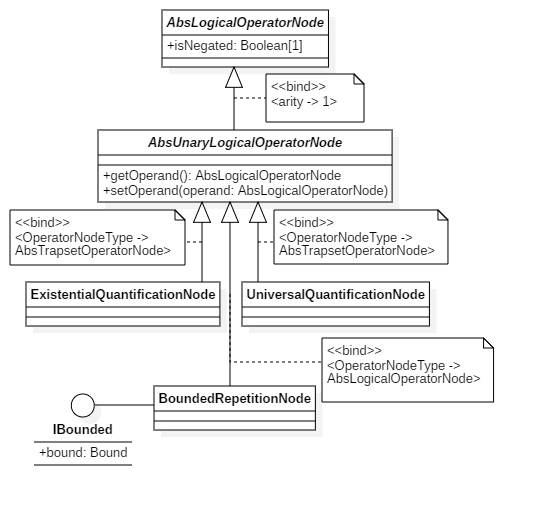
\includegraphics[width=0.95\textwidth]
			{Models/LogicalOperatorTypesUnary}
		\end{center}
		\caption{Unary logical operator types.}
		\label{fig:unary-logical-types}
	\end{figure}

	\newpage

	\par Binary logical operator types are provided below:

	\begin{figure}[h]
		\begin{center}
			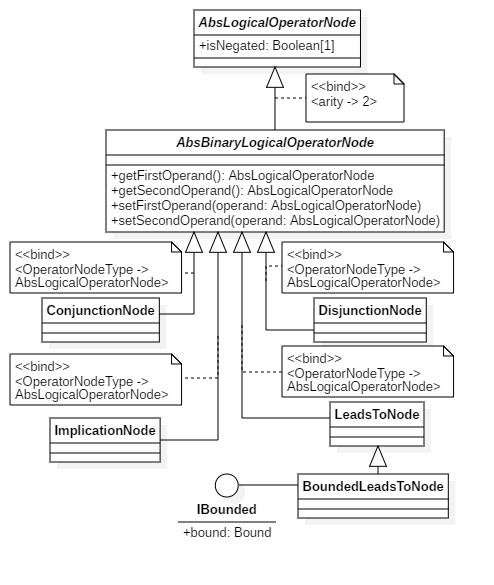
\includegraphics[width=0.8\textwidth]
			{Models/LogicalOperatorTypesBinary}
		\end{center}
		\caption{Binary logical operator types.}
		\label{fig:binary-logical-types}
	\end{figure}

	\newpage

	\par Note that we had to define two arity contract sub-classes for both\\
	\texttt{AbsTrapsetOperatorNode} and \texttt{AbsLogicalOperatorNode}. The reason for this is that it lets clients understand the API for operator types more easily. This isn't a problem with two main operator types but it will make adding operator types inconvenient in the future. In the following section we explain a work-around (hack) in the implementation language \textit{(this will look bad in the thesis)}.

	\par We also implement a visitor interface for the expression tree. This interface is based on the Visitor pattern described in \cite{patternbook}.

	\section*{Implementation}
	\par The following subsections present information on the implementation of the TDL\textsuperscript{TP} expression tree object model.

	\subsection*{Technology}
	\par Since the ANTLR-generated grammar for TDL\textsuperscript{TP} is implemented in Java, it will be easier for us to implement an adapter between the object model defined here and the ANTLR grammar object model if we implement th expression object model in Java as well.

	\subsection*{Technical Details}
	\par This section provides the most important implementation details for the expression object model.

	\subsubsection*{Arity Fix}
	\par In TDL\textsuperscript{TP}, operators can be binary or unary. In the future, it is possible that we will also need to support new operators with different arities.

	\bigskip

	\par In any case, clients should not have to infer the arity of a concrete operator implementation - this information should be encoded in the contract of the implementation.

	\newpage

	\par An approach for encoding arity information is presented in the Requirements Analysis section of this document. Its implementation in Java is presented below:

	\begin{lstlisting}[
basicstyle=\small,
caption={Arity contract approach for operator node types.},label={lst:basic-arity-contract}
]
public abstract class AbsBinaryOperator<O extends AbsExpressionNode>
  extends AbsOperatorNode<O> {
	public O getFirstOperand() {...}
	public O getSecondOperand() {...}
	...
}

public abstract class AbsUnaryOperator<O extends AbsExpressionNode>
  extends AbsOperatorNode<O> {
	public O getOperand() {...}
	...
}
	\end{lstlisting}

	\bigskip

	\par Seems like a straight-forward solution. Now let's assume that we need to subclass \texttt{AbsOperatorNode} to group concrete operator types.

	\begin{lstlisting}[
basicstyle=\small,
caption={Operator type grouping.},label={lst:operator-type-grouping}
]
public abstract class AbsLogicalOperatorNode<O extends AbsExpressionNode>
  extends AbsOperatorNode<O> {
	...
}

public abstract class AbsTrapsetOperatorNode<O extends AbsExpressionNode>
  extends AbsOperatorNode<O> {
	...
}
	\end{lstlisting}

	\bigskip

	\par Good but these classes do not have an arity contract. Let's fix it by subclassing the \texttt{Abs\textit{Type}Operator} classes:
	\begin{lstlisting}[
basicstyle=\small,
caption={Arity extension for the operator type grouping.},label={lst:operator-type-grouping-extended}
]
public abstract class AbsBinaryLogicalOperatorNode<
  O extends AbsExpressionNode> extends AbsBinaryOperator<O> {
	...
}

public abstract class AbsUnaryLogicalOperatorNode<
  O extends AbsExpressionNode> extends AbsUnaryOperator<O> {
	...
}

// AbsTrapsetOperatorNode is extended analogously
	\end{lstlisting}

	\bigskip

	\par But this way we have no \texttt{AbsLogicalOperatorNode} ancestor-class that we could generically reference. 
	Additionally, we need to have \texttt{Abs(\textit{Arity})(\textit{Type})Operator} subclasses for each \texttt{\textit{Type}} ancestor class. The solution is untenable.

	\bigskip

	\par Another approach is presented below:
	\begin{lstlisting}[
basicstyle=\small,
caption={Arity contract defined using multiple inheritance.},label={lst:multiple-inheritance}
]
public abstract class AbsLogicalOperatorNode<O extends AbsExpressionNode>
  extends AbsOperatorNode<O> {
	...
}

public abstract class AbsLogicalBinaryOperatorNode<O extends AbsExpressionNode>
  extends AbsLogicalOperatorNode<O>, AbsBinaryOperator<O> {
	...
}
public abstract class AbsLogicalUnaryOperatorNode<O extends AbsExpressionNode>
  extends AbsLogicalOperatorNode<O>, AbsUnaryOperator<O> {
	...
}
// AbsTrapsetOperatorNode is extended analogously
	\end{lstlisting}
	\bigskip 

	\par The solution in listing~\ref{lst:multiple-inheritance} is not possible because multiple inheritance is not supported in Java. Additionally, the solution suffers from the duplication issue mentioned for listing~\ref{lst:operator-type-grouping-extended} .

	\bigskip

	\newpage

	\par Our only solution is use arity interfaces that provide default implementations for arity contract methods:
	\begin{lstlisting}[
basicstyle=\small,
caption={Arity contract work-around in Java.},label={lst:multiple-inheritance}
]
public interface IOperator<O> {
	O getOperator(int ordinal);
	void setOperator(int ordinal, O operator);
}

public interface IBinaryOperator<O> extends IOperator<O> {
	default O getFirstOperator() {
		return this.getOperator(0);
	}
	default O getSecondOperator() {
		return this.getOperator(1);
	}
	...
}
	
public interface IUnaryOperator {
	default O getOperator() {
		return this.getOperator(0);
	}
}

public abstract class AbsOperatorNode<O extends AbsExpressionNode>
  extends IOperator<O> {
	...
}

public ConcreteOperator
  extends AbsOperatorNode<AbsExpressionNode>
  implements IBinaryOperator<AbsExpressionNode> {
	...
}
...
	\end{lstlisting}

	\newpage

	\par This solution allows us to simply extend \texttt{AbsOperatorNode} in our abstract sub-classes. Concrete classes should use the either the \texttt{IBinaryOperator} or the \texttt{IUnaryOperator} interface to include an arity contract. For example:
	\begin{lstlisting}[
basicstyle=\small,
caption={Arity contract work-around in Java.},label={lst:multiple-inheritance}
]
public abstract class AbsLogicalOperatorNode<O extends AbsExpressionNode>
  extends AbsOperatorNode<O> {
	...
}
public class ImplicationNode
  extends AbsLogicalOperatorNode<AbsLogicalOperatorNode>
  implements IBinaryOperator<AbsLogicalOperatorNode> {
	...
}
	\end{lstlisting}

	\par In this solution, we are simulating multiple inheritance via Java defender methods. Note that this actually goes against the intended purpose of defenders and interfaces (\cite{defaultmethodslink}).

	\bigskip

	\par The only problem is that \texttt{AbsOperatorNode} needs to have an initial arity when constructed (which it will use to initialize an operand array). Interfaces cannot fix this easily.

	\bigskip

	\par One solution is to define \texttt{IOperator.getArity()} and provide default impls in the \texttt{I(\textit{Binary|Unary})Operator} child interfaces. This way we can provide a default constructor that lacks an arity argument.

	\subsubsection*{Client-facing Classes}
	\par The remainder of this section devotes a sub-section for each client-facing class. A list of these classes is presented below:
	\begin{itemize}
		\item \texttt{ExpressionTree};
		\item \texttt{TrapsetSymbolNode};
		\item \texttt{AbsoluteComplementNode};
		\item \texttt{LinkedPairNode};
		\item \texttt{RelativeComplementNode};
		\item \texttt{UniversalQuantificationNode};
		\item \texttt{ExistentialQuantificationNode};
		\item \texttt{Bound};
		\item \texttt{EBoundType};
		\item \texttt{BoundedRepetitionNode};
		\item \texttt{ConjunctionNode};
		\item \texttt{DisjunctionNode};
		\item \texttt{ImplicationNode};
		\item \texttt{LeadsToNode};
		\item \texttt{BoundedLeadsToNode};
		\item \texttt{IExpressionTreeVisitor};
		\item \texttt{BaseExpressionTreeVisitor}.
	\end{itemize}
BaseExpressionTreeVisitor
	\subsubsection{\texttt{}}

	\printbibliography[
		title=Sources
	]

\end{document}
